\chapter{Arquitectura}
En este capitulos se detallara la arquitectura del proyecto en general, poniendo foco en la seleccion adecuada de las tecnologias a utilizar y completando mas detalladamente el diseño obtenida en el capitulo anterior.

\section{Procesador Embebido}

Como se dijo en el capitulo 2, los microprocesadores embebidos en logica reprogramable se clasifican, basicamente, en dos tipos Hardcore y Softcore. Aunque los Hardcores ofrecen unas mejores prestaciones existen muy pocos dispositivos en el mercado que ofrecen este tipo de modulos y, en general, el costo de este tipo de dispositivos es mayor que el de uno que no cuenta con un hardcore. Por esta razones de ahora en adelante se limitara el estudio a softcores, siempre buscando que lo implementado siga los principios del diseño modular a los fines de facilitar la portabilidad.
\subsection{Estudio de los softcores disponibles}
Los SoftCores pueden ser clasificados en tres tipos segun su origen

\begin{itemize}
	\item Provistos por los fabricantes de las FPGA
	\item Provistos por empresas distribuidoras de bloques IP(Intelectual Property)
	\item Provistos por la comunidad Open Source
\end{itemize}

\subsubsection{Provistos por los fabricantes de las FPGA}
Xilinx y Altera, los dos mayores fabricantes de FPGA, proveen un Softcore para integrar en sus dispositivos. La ventaja natural de este tipo de core es que se encuentran altamente integrados en las herramientas de desarrollo de dichos fabricantes, permitiendo montar un sistema embebido en minutos de manera grafica e intuitiva. Ademas estan a disposición del usuario una buena cantidad de  modulos IP para anexar al procesador y aumentar asi sus funcionalidades. 

Dentro de las desventajas esta el hecho de que son dependientes de la plataforma y no es posible implementar el core propietario de Altera en un dispositivo Xilinx, y viseversa. Ademas se debe pagar una licencia por el uso de estos cores y no se cuenta con la posibilidad de observar o modificar el codigo de los mismos. 

Xilinx ofrece a los usuarios de sus dispositivos el MicroBlaze, un procesador RISC de 32 bits con una arquitectura muy similar al MIPS DLX. A nivel herramientas de desarrollo la empresa provee el "Xilinx's EDK(Embedded Development Kit)" que permite generar un sistema embebido completo con las interconexiones necesarias. Es posible correr el sistema operativo GNU/Linux en este tipo de procesador.

Altera por su parte ofrece la linea de Cores NIOS II, tambien RISC de 32 bits, que cuenta en tres variantes principales Nios II Fast, Economy y Standard y dos variantes especializadas Nios II SC core, para aplicaciones militares y aeroespaciales, y DesignWare IP, para implementar en ASIC. Altera provee ademas una interfaz de usuario para la construccion del sistema embebido llamado SOPC que se encuentra integrado a Quartus y ademas el Nios II Embedded Design Suite (EDS) que permite diseñar el software requerido para cada aplicacio. Permite la implementacion del sistema operativo GNU/Linux.

\subsubsection{Provistos por empresas distribuidoras de bloques IP}
Existe una buena cantidad de empresas que se dedican a generar y comercializar bloques de propiedad intelectual (IP Cores o IP Blocks), unidades logicas reusables que son propiedad intelectual de un individuo o empresa.
Varias de estas empresas cuentan con Softcores con distintas capacidades y tecnologias. La ventaja principal esla portabilidad de estos cores entre FPGA de distintos fabricantes. Entre las desventajas podemos nombrar la calidad de la documentacion y la complejidad intrinseca que implica comprender y utilizar una herramienta de desarrollo de un tercero. 

Dentro de los mas conocidos se puede nombrar a la linea Leon de la empresa Aeroflex, LatticeMico32 de Lattice semiconductor o ARM cortex de Freescale. Los IP core pueden estar licenciados de diferentes formas incluidas entre ellas GPL.
 
\subsubsection{Provistos por la comunidad Open Source}
La comunidad open source se ha encargado de producir una buena cantidad de softcores, las capacidades y perfomance de los mismos cubre casi todos los rangos. En la pagina web que lleva una lista de este tipo de proyectos, opencores, se pueden encontrar alrededor de 130 cores. El problema con este tipo de core esta en la poco uniforme calidad de la documentacion y en la calidad dudosa de varios de los cores. Sin embargo la flexibilidad para poder modificar la arquitectura a gusto y el costo cero de implementacion son ventajas nada despreciables de estos productos. 

Se destaca el proyecto Openrisc 1200, que tiene una gran comunidad que lo soporta y algun prestigio ganado en este terreno.


\subsubsection{Tabla comparativa}
																																						 \newpage																												
\begin{table}


	\centering
	\begin{tabular}{|p{1.65cm}|p{1.98cm}|c|p{2.2cm}|p{1.5cm}|c|c|p{1.5cm}|} \hline
		Core & Arquitectura & Licencia & Profundidad del Pipeline & Ciclos por Instruccion & MMU & FPU & FPGA \\ \hline
		MicroBlaze & MicroBlaze & Propietaria & 3,5 & 1 & Opt & Opt & Xilinx\\ \hline
		Nios II/fast & Nios II & Propietaria & 6 & 1 & si & opt & Altera \\ \hline
		Nios II/std & Nios II & Propietaria & 5 & 1 & no & Opt & Altera \\ \hline
		Nios II/econ & Nios II & Propietaria & no & 6 & no & Opt & Altera \\ \hline
		LEON3 & SPARC-v8 & GPL & 7 & 1 & si & si & Xilinx, Altera, Lattice \\ \hline
		OpenRISC 1200 & OpenRISC 1000 & LGPL & 5 & 1 & si & no & Xilinx, Altera, Lattice \\ \hline
		Lattice Mico32 & Lattice Mico32 & Propietaria & 6 & 1 & no & no & Indep. \\ \hline
		Cortex-M1 & ARMv6 & Propietaria & 3 & 1 & no & no & Xilinx, Altera \\ \hline
	\end{tabular}
	\caption{Comparativa softcores}
	\label{tab:comp}
\end{table}

\subsection{Criterios de Seleccion}

Los criterios mas importantes a la hora de seleccionar el Softcore que va a ser utilizado en este proyecto son:
\begin{itemize}
	\item Hardware: se debe contar con el dispositivo necesario para la implementacion de estos dispositivos.
	\item Herramientas de Diseño: la cadena de herramientas necesarias para diseñar el sistema y el software debe ser simple y funcional, para evitar que comprender las herramientas lleve mas tiempo que realizar el proyecto en si mismo.
	\item Rendimiento: se desea que el rendimiento sea aceptable y que sea posible optimizarlo a medida de que el proyecto avanza.
\end{itemize}

Bajo estos criterios y teniendo en cuenta que en el laboratorio en que se realiza el presente proyecto integrador es posible acceder a una amplia variedad de kits de desarrollo equipados con FPGAs de Altera, todas las licencias de software y varios proyectos con antencedentes de haber puesto en funcionamiento un Nios II es este el Core seleccionado para el sistema embebido a implementar.

\subsection{Nios II}
El Nios II es un procesador RISC de 32 bits de proposito general que cuenta con las siguientes especificaciones:
\begin{itemize}
	\item Set de instrucciones, bus de datos y espacio de direcciones de 32 bits.
	\item 32 registros de proposito general.
	\item Soporte para hasta 32 interrupciones.
	\item Controlador de interrupciones externas para soportar una mayor cantidad de interrupciones.
	\item Multiplicacion y division en una sola instruccion de 32 x 32 produciendo un resultado de 32-bits.
	\item Instrucciones dedicadas para multiplicaciones con resultados de 64 y 128 bits.
	\item Acceso a una variedad de perifericos e interfases a memorias  y perifericos fuera del chip.
	\item Modulo de depurado asistido por hardware.
	\item Unidad de manejo de memoria (MMU) opcional para soportar sistemas operativos mas complejos.
	\item Unidad de proteccion de memoria (MPU) opcional.
	\item Entorno de desarrollo de software basado en GNU C/C++ integrado a Eclipse.
	\item Integracion con SignalTap® II, el analizador de logica embebida de altera permitiendo el analisis de tiempo real de todas las señales presentes en la FPGA.
	\item Set de instrucciones compatible entre todos las versiones del procesador Nios II.
\end{itemize}


\subsection{SOPC}
\section{Modulo Gestor de Datos}
\section{Software}

\subsection{NIOS II SBT}

El NIOS II Software Building Tools (o SBT) es un conjunto de utilidades y scripts que sirve para crear y construir aplicaciones embebidas basadas en C/C++, librerías de usuario y paquetes de soporte de placa (board support packages o BSP). 

Puede invocarse desde la IDE Eclipse o desde el intérprete de comandos del NIOS II.

El NIOS II SBT puede crear los siguientes tipos de proyecto:
\begin{itemize}
	\item Aplicación NIOS II: un programa que implementa alguna funcion deseada.
	\item NIOS II BSP: una librería que provee acceso al hardware en el sistema. Brinda un entorno de rutinas a medida para un procesador y, eventualmente, un sistema operativo. 
	\item Librería de usuario: un conjunto de funciones reutilizables. 
\end{itemize}

\subsubsection{Aplicaciones y librerías de usuario}

Para el caso de aplicaciones y librerías de usuario, el SBT genera un makefile privado (denominado \textbf{Makefile}) el cual es usado para construir el proyecto. Al hacer esto se genera un archivo .elf para una aplicación, o .a para una librería. En este último caso, también se produce un makefile público (denominado \textbf{public.mk}), que se incluye en el privado para cualquier aplicación que use la librería de usuario.

Cuando se crea un makefile se provee al SBT con una lista de archivos de código fuente y una referencia al directorio donde se almacena el BSP. Luego, la herramienta examina la extensión de cada archivo fuente para determinar el lenguaje de programación. 

Actualmente, los soportados son:

\begin{itemize}
	\item C (extensión .c).
	\item C++ (extensiones .cpp, .cxx, .cc).
	\item NIOS II Assembler (extensiones .s, .S).
\end{itemize}


\subsubsection{Board Support Packages}

Un BSP es una librería especializada que contiene código de soporte específico del sistema. Aisla la aplicación de los detalles del sistema, tales como mapeo de memoria, dispositivos disponibles y configuración del procesador.

Se compone de:

\begin{itemize}
	\item Capa de abstracción de Hardware (Hardware Abstraction Layer o HAL): Permite al software interactuar con el hardware del sistema. Se describirá en detalle más adelante en este capítulo.
	\item Librería C estándar newlib: ANSI C estándar diseñada para sistemas embebidos.
	\item Drivers de dispositivos: para manejar cada uno de los componentes del sistema.
	\item Paquetes de software opcionales: permiten proveer funcionalidad adicional.
	\item Sistema operativo de tiempo real opcional: implementación de MicroC/OS-II RTOS.
\end{itemize}

\subsubsection{Proceso de construcción del software}

Para crear un proyecto de software se llevan a cabo una serie de pasos:

\begin{enumerate}
	\item Se obtiene el diseño de hardware sobre el cual va a correr el software. Dicha información está almacenada en un archivo de extensión \textbf{.sopcinfo}, el cual es generado por la herramienta SOPC builder.
	\item Se genera el BSP con las características necesarias según las funcionalidades requeridas. También se genera un makefile para dicho paquete.
	\item Opcionalmente, se crea una librería de usuario (junto a su correspondiente makefile).
	\item Se escribe el software de aplicación. Se colecta todo el código fuente, y luego se genera el makefile correspondiente.
	\item Se construye el proyecto.
\end{enumerate}


\subsection {HAL}

La Capa de Abstracción de Hardware \textit{(Hardware Abstraction Layer o HAL)} provee una interfaz simple de drivers de dispositivos para conectar los programas con el hardware subyacente. La API está integrada con la librería estándar ANSI C, lo cual permite al software acceder a los dispositivos mediante el uso de funciones C ampliamente conocidas, tal como printf(), fopen(), fwrite(), etc.

\subsubsection{Servicios}

La HAL provee los siguientes servicios:

\begin{itemize}
	\item Integración con la librería estándar newlib: provee funciones estándar ANSI C de amplio uso.
	\item Drivers de dispositivo: brinda acceso a cada dispositivo en el sistema.
	\item API: proporciona una interfaz estándar consistente a los servicios de la HAL, tales como acceso a dispositivos y manejo de interrupciones.
	\item Inicialización de sistema: Lleva a cabo la inicialización para el procesador y las rutinas antes de ejecutar la función principal (main).
	\item Inicialización de dispositivos: Instancia e inicializa cada uno de los dispositivos del sistema antes de que se ejecute la función main.
\end{itemize}

La figura ~\ref{fig:hal} muestra las capas de un sistema basado en la HAL, desde el nivel de hardware hasta el programa de usuario.

\begin{figure}[H]
  \centering
	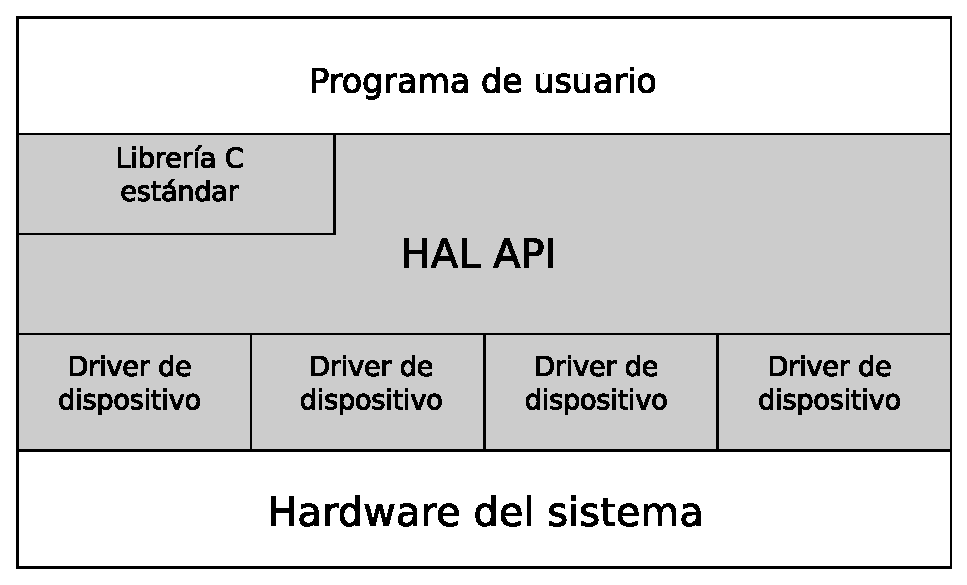
\includegraphics[width=0.80\textwidth]{3-arquitectura/graf/hal.eps}
  \caption{Capas de un sistema basado en la HAL.}
  \label{fig:hal}
\end{figure}

\subsubsection{Modelos de dispositivos genéricos}

La HAL provee modelos de dispositivos genéricos para diversos tipos de periféricos que se encuentran en sistemas embebidos, tales como timers, interfaces Ethernet y dispositivos de I/O que transmiten datos de caracter. Estos modelos permiten escribir programas usando una API consistente sin preocuparse por el hardware subyacente.

Los tipos de periféricos cubiertos son:

\begin{itemize}
	\item Dispositivos de caracter: envían y/o reciben caracteres en forma serial, como ser una UART.
	\item Timers: dispositivos que llevan la cuenta de los tics de un clock y pueden generar interrupciones periódicas.
	\item Subsistemas de archivos: un mecanismo para acceder a archivos almacenados en dispositivos físicos. Dependiendo de la implementación interna, el driver del subsistema de archivos podría acceder a los dispositivos subyacentes en forma directa o usar un driver aparte.
	\item Dispositivos Ethernet: proveen acceso a una conexión Ethernet para una pila de red, tal como la NicheStack® TCP/IP Stack, provista por Altera.
	\item Dispositivos DMA: periféricos que llevan a cabo una gran cantidad de transacciones de datos. El origen y destino pueden ser la propia memoria o algún otro dispositivo.
	\item Dispositivos con memoria flash: periféricos con memoria no volátil que utilizan un protocolo especial de programación para almacenar datos.
\end{itemize}

Todos los periféricos, ya sean de Altera o de terceros, deben proveer un archivo de cabecera que defina la interfaz de bajo nivel del dispositivo con el hardware. 

Ciertos dispositivos tienen características específicas de hardware con requierimientos de uso que no se adaptan bien a una API de propósito general. La HAL maneja dichos requerimientos mediante la función ioctl(), cuyas opciones dependerán del periférico en cuestión.

Algunos periféricos proveen funciones de acceso dedicadas que no están basadas en el modelo genérico de la HAL. En ese caso, se debe proveer un archivo de cabecera con dichas funciones.


\subsubsection{Librería C estándar : newlib}
La HAL integra su entorno de rutinas con una implementación open-source de la librería C estándar:\textbf{ newlib}. La misma está hecha para ser utilizada en sistemas embebidos. 

\subsubsection{La HAL dentro de un proyecto de software}
La creación y administración de proyectos basados en la HAL están altamente ligadas al NIOS II SBT

\begin{figure}[h]
  \centering
	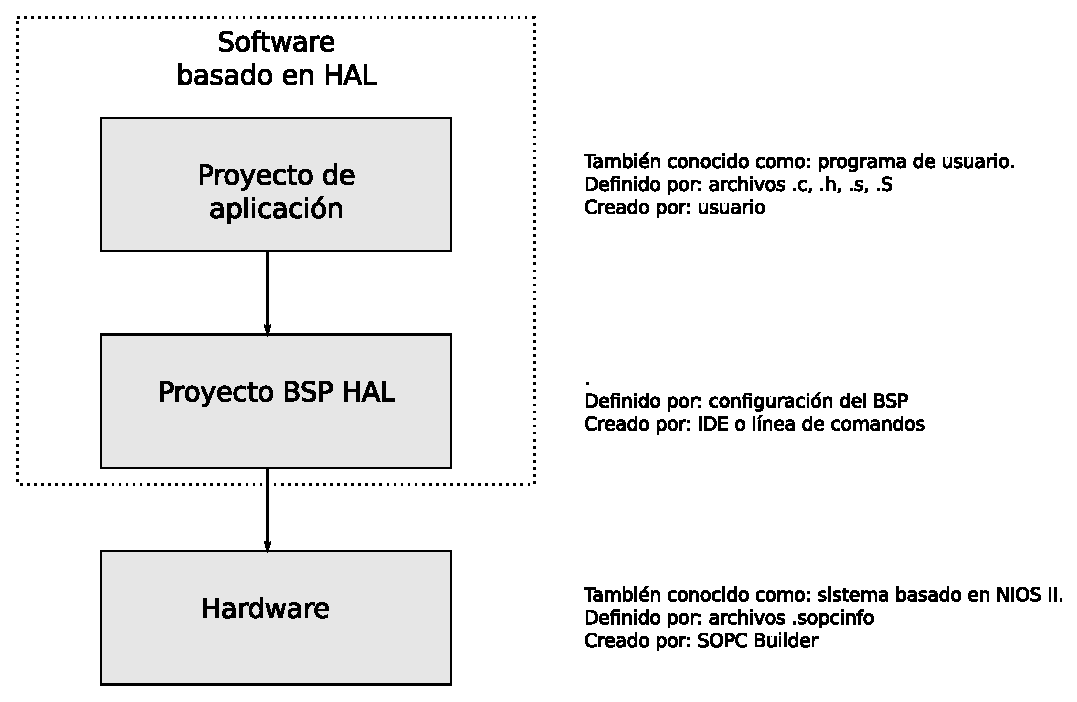
\includegraphics[width=0.90\textwidth]{3-arquitectura/graf/halsof.eps}
  \caption{Capas de un programa basado en HAL}
  \label{fig:halsof}
\end{figure}

La figura ~\ref{fig:halsof} muestra el diagrama en bloques de un software basado en la HAL. Todo programa de este tipo consta de dos proyectos. El ćodigo de aplicación específico se encuentra en uno de ellos, el cual depende a su vez de otro proyecto BSP separado.

EL primero contiene todo el código que el programador desarrolla. El segundo, toda la información necesaria para la interacción hardware-software. Este último a su vez depende del hardware del sistema, cuya información se encuentra en un archivo generado por la herramienta SOPC Builder.

\subsubsection{El archivo de descripción del sistema (system.h)}
El archivo system.h provee una descripción completa del software del sistema basado en NIOS II. Describe cada periférico e incluye:

\begin{itemize}
	\item La configuración de hardware del periférico.
	\item La dirección base.
	\item Información IRQ (si es necesario).
	\item Un nombre simbólico para el periférico.
\end{itemize}

El SBT genera un archivo \textbf{system.h} para cada proyecto BSP, cuyo contenido dependerá del archivo .sopcinfo mencionado anteriormente en este capítulo.

\subsubsection{Acceso al hardware}
El software accede al hardware a través de macros que abstraen la interfaz mapeada en memoria al dispositivo. Todos los componentes proveen un directorio que define el hardware y el software del periférico en cuestión. En esta carpeta se encuentra un archivo de cabecera que define la interfaz con el hardware y su nombre es $<componente>$\_regs.h, el cual se incluye en el subdirectorio inc. Por ejemplo, el componente JTAG UART define su interfaz en el archivo $<Directorio Instalacion Altera>$/ip/altera/sopc\_builder\_ip/

altera\_avalon\_jtag\_uart/inc/altera\_avalon\_jtag\_uart\_regs.h.

El archivo de cabecera \_regs.h define las siguientes macros de acceso para el componente:
\begin{itemize}
	\item Macros de acceso a registros que proveen operaciones de lectura/escritura. Éstas son:
	\begin{itemize}
		\item IORD\_$<NombreDelComponente>$\_$<NombreDelRegistro>$ ($<DireccionBaseDelComponente>$).
		\item IOWR\_$<NombreDelComponente>$\_$<NombreDelRegistro>$ ($<DireccionBaseDelComponente>$, $<Dato>$).
	\end{itemize}
	\item Macros de direccionamiento de registro, que retornan las direcciones físicas de cada uno de ellos. La dirección devuelta es la dirección base del componente + el valor de desplazamiento de registro especificado. Esta macro tiene el nombre de esta forma:
	\begin{itemize}
		\item IOADDR\_$<NombreDelComponente>$\_$<NombreDelRegistro>$ ($<DireccionBaseDelComponente>$).
	\end{itemize}
	\item Máscaras a nivel de bits. Estas macros tienen los siguientes nombres:
	\begin{itemize}
		\item $<NombreDelComponente>$\_$<NombreDelRegistro>$\_$<NombreDelCampo>$\_MSK : Máscara de bit de un campo.
		\item $<NombreDelComponente>$\_$<NombreDelRegistro>$\_$<NombreDelCampo>$\_OFST : Desplazamiento de bit del el comienzo del campo.
	\end{itemize}
\end{itemize}

Cabe mencionar que las los valores leídos/escritos mediante las macros de acceso a registro (IORD e IOWR) no trabajan con la caché del microprocesador.



La razón de utilizar la HAL en vez de un sistema operativo, yace principalmente en la mayor simplicidad de uso que ésta presenta. En el caso de haber optado por el segundo enfoque hubiese sido necesario el desarrollo de drivers para el manejo de los dispositivos, con la complejidad que ello implica. La HAL, por otra parte, ofrece un conjunto de funciones de la librería estándar ANSI C para la interacción con el hardware del diseño, lo cual hace que dicha tarea sea significativamente más simple.



\subsection {Algoritmos de clasificación}

Se implementaron 2 algoritmos de clasificacion: Busqueda lineal y Busqueda en árbol unibit.

El software utilizado para realizar las pruebas consistió en 2 proyectos por separado. Uno para cada tipo de búsqueda en la tabla.

El mismo fue desarrollado en lenguaje c++, por presentar éste ciertas facilidades para las implementaciones llevadas a cabo. Puntualmente se sacó ventaja de un STL container (list) para implementar la búsqueda lineal. La característica utilizada en este caso fue el ordenamiento de la lista con sólo una llamada a función.

Para efectuar el intercambio de datos con el hardware se hizo uso de las macros IOWR e IORD, las cuales escriben y leen respectivamente los datos hacia/desde un componente conectado al bus Avalon MM. La razón de haber usado dichas macros yace en el hecho de que las mismas no son puestas en caché. Esta característica se torna indispensable en este diseño, ya que en el mismo no se puede leer un dato sin saber si está verdaderamente disponible en el bus.


\subsubsection {Búsqueda lineal}

Se implementó en una lista enlazada, creada a partir del template list de c++. Los nodos de la lista contienen 3 campos:

\begin{itemize}
	\item Dirección de red (entero de 32 bit sin signo)
	\item Máscara de red (entero de 32 bit sin signo)
	\item Identificador de decisión (entero de 32 bit con signo)
\end{itemize}

Como se le dió prioridad a los prefijos de red más largos, se debió sobrecargar el operador de comparación ( > ) para que la función sort pudiese ordenar en base a la longitud de máscara. De esa manera, los nodos que contenían valores de máscara más grandes quedaban en las primeras posiciones de la lista.

Cuando la función encargada del lookup recibe una dirección IP de destino, realiza los siguientes pasos:

\begin{itemize}
	\item Coloca un iterador al comienzo de la lista.
	\item Realiza un AND con el valor de máscara del nodo que está siendo apuntado. Si el resultado de la operación es igual al valor de dirección de red de dicho nodo, entonces se retorna con el valor identificador de decisión. En otro caso, continúa la busqueda en el siguiente nodo.
\end{itemize}

\subsubsection {Busqueda en Arbol unibit}

Se implementó una clase en la cual se definieron las características de los nodos del arbol, como así tambien las operaciones de inserción y búsqueda.

En este contexto, pueden existir 2 tipos de nodo:

\begin{itemize}
	\item Común: no está asociado a una decisión.
	\item Decisión: contiene un valor que identifica a la decisión a tomar. 
\end{itemize}

Cada nodo cuenta con los siguientes campos:
\begin{itemize}
	\item gw: es un identificador de la decisión a tomar. En los nodos no asociados a una decision, tiene el valor estipulado en la macro NONE.
    \item zero / one: Son punteros a nodo, asociados a los bits 0/1 del prefijo que se esté leyendo.

\end{itemize}




El algoritmo de búsqueda toma como entrada la dirección IP de destino del paquete a clasificar. Luego de ello, va haciendo un testeo bit a bit de la misma, partiendo con un puntero de recorrido desde el nodo raíz. Si el bit de la dirección es 0 y el puntero zero está apuntando hacia algun nodo, el puntero de recorrido se mueve al nodo apuntado por el puntero zero. En caso contrario, se mueve al nodo apuntado por el puntero one (En caso de que exista alguno). Esto se repite nodo a nodo, hasta que ocurre alguna de las siguientes situaciones:

\begin{itemize}
    	\item     El puntero de recorrido queda varado en un nodo decision, con lo cual se retorna el valor de gw.
    	\item El puntero de recorrido queda varado en un nodo común. 
\end{itemize}



Contemplando esta última posibilidad, el algoritmo hace que en cada nodo se chequee si se trata de un nodo decisión. En dicho caso, se almacena el campo gw en una variable y se continua el recorrido. Si se da un caso en el cual el nodo de recorrido queda apuntando a un nodo comun y luego de testear un bit se determina que el mismo no tiene un nodo asociado (es decir, que alguno de los punteros zero / one esté en NULL) la funcion retorna la variable anteriormente mencionada. 

\subsection {Cache}

Se implementó una cache directa. La misma consta de una tabla hash de 16 entradas. Las colisiones se resuelven por reemplazo directo. La misma fue testeada con ambos algoritmos mencionados anteriormente. Para ello, se agregó una lógica adicional que consistió en:

\begin{itemize}
	\item Al tomar una direccion IP, chequear primero si el valor de decisión se encuentra en caché.
	\item Si está, retornar dicho valor.
	\item En otro caso, efectuar el lookup y almacenar el valor de decisión en caché.
\end{itemize}

Para evitar el overhead introducido por el uso de clases, se optó por el uso de estructuras para la implementación de este último enfoque.

\begin{comment}
\section{Parte HW}

\subsection{Componentes del sistema}

\subsubsection*{NIOS II}

Es un microprocesador softcore. Esto significa que el mismo es instanciado usando la lógica propia de la FPGA. En este diseño, ejecuta un software de clasificación de paquetes que se almacena en una memoria SDRAM en la placa de desarrollo.

\subsubsection*{PLL}

Este módulo toma como entrada una señal de clocl de 50 MHZ de frecuencia y la bifurca en 2: Una de ellas alimentará al módulo que oficia de interfaz con la memoria SDRAM y la otra hará lo propio con el resto de los componentes del sistema. Estas señales están defasadas entre sí 60º con el fin de evitar el skew producido por la diferencia entre la llegada del clock a la memoria y al resto del sistema.

\subsubsection*{Timer}

Módulo utilizado para llevar estadísticas de retardo dentro del software.

\subsubsection*{JTAG UART}

Este módulo permite interactuar con el sistema vía USB. Esto implica tanto la configuracion de la FPGA, como también la posibilidad de ver la ejecución del software en una consola.

\subsubsection*{Interfaz con SDRAM}

Tiene la función de interconectar al sistema con la memoria SDRAM de la placa de desarrollo.

\subsubsection*{Extractor de cabeceras}

Este módulo extrae cabeceras de paquetes Ethernet y las envía al software, donde son procesadas y devueltas. Su funcionamiento se detallará a continuación.

\subsection{Módulo extractor de cabeceras}


(..esta parte completala vos...)

\section{Parte SW}

\section{Parte SW}

Se implementaron 2 algoritmos de clasificacion: Busqueda lineal y Busqueda en árbol unibit.

El software utilizado para realizar las pruebas consistió en 2 proyectos por separado. Uno para cada tipo de búsqueda en la tabla.

El mismo fue desarrollado en lenguaje c++, por presentar éste ciertas facilidades para las implementaciones llevadas a cabo. Puntualmente se sacó ventaja de un STL container (list) para implementar la búsqueda lineal. Esta plantilla cuenta con, entre otras cosas, la posibilidad de ordenar la lista con sólo una llamada a función.

Para efectuar el intercambio de datos con el hardware se hizo uso de las macros IOWR e IORD, las cuales escriben y leen respectivamente los datos hacia/desde un componente conectado al bus Avalon MM. La razón de haber usado dichas macros yace en el hecho de que las mismas no son "cacheadas". Esta característica se torna indispensable en este diseño, ya que en el mismo no se puede leer un dato sin saber si está verdaderamente disponible en el bus.


\subsection {Búsqueda lineal}

Se implementó en una lista enlazada, creada a partir del template list de c++. Los nodos de la lista contienen 3 campos:

\begin{itemize}
	\item Dirección de red (entero de 32 bit sin signo)

	\item Máscara de red (entero de 32 bit sin signo)

	\item Identificador de decisión (entero de 32 bit con signo)
\end{itemize}

Como se le dió prioridad a los prefijos de red más largos, se debió sobrecargar el operador de comparación ( > ) para que la función sort pudiese ordenar en base a la longitud de máscara. De esa manera, los nodos que contenían valores de máscara más grandes quedaban en las primeras posiciones de la lista.

Cuando la función encargada del lookup recibe una dirección IP de destino, realiza los siguientes pasos:

\begin{itemize}
	\item Coloca un iterador al comienzo de la lista.
	\item Realiza un AND con el valor de máscara del nodo que está siendo apuntado. Si el resultado de la operación es igual al valor de dirección de red de dicho nodo, entonces se retorna con el valor identificador de decisión. En otro caso, continúa la busqueda en el siguiente nodo.
\end{itemize}

\subsection {Busqueda en Arbol unibit}

Se implementó una clase en la cual se definieron las características de los nodos del arbol, como así tambien las operaciones de inserción y búsqueda.
Cada nodo cuenta con los siguientes campos:
\begin{itemize}
	\item gw: es un identificador de la decisión a tomar. En los nodos no asociados a una decision, tiene el valor estipulado en la macro NONE.
    \item zero / one: Son punteros a nodo, asociados a los bits 0/1 del prefijo que se esté leyendo.

\end{itemize}

En este contexto, pueden existir 2 tipos de nodo:

\begin{itemize}
	\item Común: Está asociado a la macro NONE. La misma lo diferencia del nodo decisión.
	\item Decisión: Contiene en el campo gw un valor que identifica a la decisión a tomar. 
\end{itemize}



El algoritmo de búsqueda toma como entrada la dirección IP de destino del paquete a clasificar. Luego de ello, va haciendo un testeo bit a bit de la misma, partiendo con un puntero de recorrido desde el nodo raíz. Si el bit de la dirección es 0 y el puntero zero está apuntando hacia algun nodo, el puntero de recorrido se mueve al nodo apuntado por el puntero zero. En caso contrario, se mueve al nodo apuntado por one (En caso de que exista). Esto se repite nodo a nodo, hasta que:

\begin{itemize}
    	\item     El puntero de recorrido queda varado en un nodo decision, con lo cual se retorna el valor de gw. Ó
    	\item El puntero de recorrido queda varado en un nodo común. 
\end{itemize}



Contemplando esta última posibilidad, el algoritmo hace que en cada nodo se chequee si se trata de un nodo decisión. En dicho caso, se almacena el campo gw en una variable y se continua el recorrido. Si se da un caso en el cual el nodo de recorrido queda apuntando a un nodo comun y luego de testear un bit se determina que el mismo no tiene un nodo asociado (es decir, que alguno de los punteros zero / one esté en NULL) la funcion retorna la variable anteriormente mencionada. 

\subsection {Cache}

Se implementó una cache directa. La misma consta de una tabla hash de 16 entradas. Las colisiones se resuelven por reemplazo directo. La misma fue testeada con ambos algoritmos mencionados anteriormente. Para ello, se agregó una lógica adicional que consistió en:

\begin{itemize}
	\item Al tomar una direccion IP, chequear primero si el valor de decisión se encuentra en caché.
	\item Si está, retornar dicho valor.
	\item En otro caso, efectuar el lookup y almacenar el valor de decisión en caché.
\end{itemize}
\end{comment}

%\section{Distribucion Lineal}
